\documentclass[a4j,12pt]{gradthesis_utf8}
%\usepackage[dviout]{graphicx}
\usepackage[dvipdfmx]{graphicx}
\usepackage{graphicx}
%\usepackage{algorithmic}
\usepackage{listings}
\usepackage{algpseudocode, algorithm}
\usepackage{url}

\usepackage{indentfirst}
%
%%% ドラフトモード(図表は,図表のみのページになる)
%\draftmode
%
%%% 2ページ目に英語の題目をいれる
\engtitle
%
%%% 2ページ目に英語の所属をいれる
\engaffil
%
%%% 2ページ目に英語の著者名をいれる
\engauthor
%
%%% ヘッダ(章番号と章タイトル)を入れる
\usehead
%
\jtitle{TCP並列接続を用いたプログレッシブダウンロード\\における順序制御方式の実装} % 和文題目
%
\etitle{Implementation of sequence control method in progressive download using TCP parallel connection} % 英文題目
%
\jaffil{広島市立大学 情報科学部 情報工学科}
\eaffil{Department of Computer and Network Engineering\\
Faculty of Information Sciences\\
Hiroshima City University}
%
\jauthor{1420180 \quad 平城 光雄} % 和文著者名
\eauthor{1420180 \quad Mitsuo Heijo} % 英文著者名
\supervisor{舟坂 淳一}  % 指導教官名
%
%
\jabst{ % 和文梗概 
\hspace*{0.5em}概要
} %

\eabst{ % 英文梗概
\hspace*{1em}gaiyo}

\begin{document} 
\maketitle %とびらの出力

%%%%%%%%%%%%%%%%%%%%%%%%%%%%%%%%%%%%%%%%%%%%%%%%%%%%%%%%%%%%%%%%%%%%%%%%%%%%%
% 第1章
%%%%%%%%%%%%%%%%%%%%%%%%%%%%%%%%%%%%%%%%%%%%%%%%%%%%%%%%%%%%%%%%%%%%%%%%%%%%%
\chapter{はじめに}\label{sec:sec1}
%%% abst %%%
はじめに
%%%%%%%%%%%%%%%%%%%%%%%%%%%%%%%%%%%%%%%%%%%%%%%%%%%%%%%%%%%%%%%%%%%%%%%%%%%%%
% 第2章
%%%%%%%%%%%%%%%%%%%%%%%%%%%%%%%%%%%%%%%%%%%%%%%%%%%%%%%%%%%%%%%%%%%%%%%%%%%%%
\chapter{関連研究}\label{sec:sec2}
本章ではまず,動画配信方式の一つであるプログレッシブダウンロードについて述べる.

\section{プログレッシブダウンロード方式}
ネットワークの大容量化,高速化に伴い,Youtube[]やNetflix[]などの動画配信サービスの利用が増加している.動画配信サービスにはUDPを利用したストリーミング,TCPを利用したプログレッシブダウンロードの2種類がある.アプリケーションプロトコルとしてHTTPを用いるプログレッシブダウンロードは特別なソフトウェアを必要とせず,ブラウザだけで視聴することができるため,近年広く普及してきている.また,プログレッシブダウンロードは分割順次ダウンロードとも呼称される.プログレッシブダウンロードの動作概要は,まず,1つのファイルを複数のあるサイズののブロックに分割する.次に,クライアントは分割されたブロックをサーバーに対してリクエストする.このリクエストの方法にはHTTPのRange Headerに分割のための情報を含める方式やHTTPのGETリクエストのクエリストリングに分割のための情報を含める方式などがある.サーバーはリクエストに応じたブロックを送信する.これを繰り返すことで,1つのファイルを取得できる.

%%%%%%%%%%%%%%%%%%%%%%%%%%%%%%%%%%%%%%%%%%%%%%%%%%%
%%%%%%%%%%%%%%%%%%%%%%%%%%%%%%%%%%%%%%%%%%%%%%%%%%%
 \section{複数経路を用いた通信方式}
 複数のIP接続を束ねて上位層に機能を提供することを目的としたものの一つのMPTCP[]などが提案されている.複数のNICを束ねることで上位層からは1つの仮想的なインターフェースとして扱うことができ,アプリケーションを限定しない汎用性がある一方で.各OSレベルでの実装が必要となるので実装コストは高い.
 

%%%%%%%%%%%%%%%%%%%%%%%%%%%%%%%%%%%%%%%%%%%%%%%%%%%%%%%%%%%%%%%%%%
 \section{複数のTCP接続を用いたプログレッシブダウンロード}
 \label{hukusu}
 ネットワークの発展に伴い,大容量のデータをTCPを用いて,通信する機会が増加しつつある.TCPには輻輳回避のためにウィンドウ制御が存在する.このため,ウィンドウサイズを遅延で割ったものが単一TCP接続における理論最大性能となる.近年ではコンテンツの大容量化が進んでおり,より効率よくコンテンツをダウンロードするためにアプリケーション層から複数のTCP接続を用いる手法が提案されている.図\ref{block}は複数のTCPを接続を用いたプログレッシブダウンロードの分割されたブロックの受信の様子を示した例である.複数のブロックを性能の異なる別々のTCP接続に対して要求を行う場合,ブロックの再生順番と受信完了順序が一致しない可能性がある.図\ref{block}が示すように,先頭から連続するブロック1及びブロック2は再生可能である(有効ブロック)が,それ以外のブロック3及びブロック5は未受信のブロックを間に挟んでいるため再生することはできない(非有効ブロック).複数のTCP接続を束ねることでグッドプットを向上させても,受信ブロックが有効ブロックでない限りは応答性は低下してしまい,動画の再生が停止するなどしてユーザー体験は悪化することが予想できる.
\begin{figure}[h]
\centering
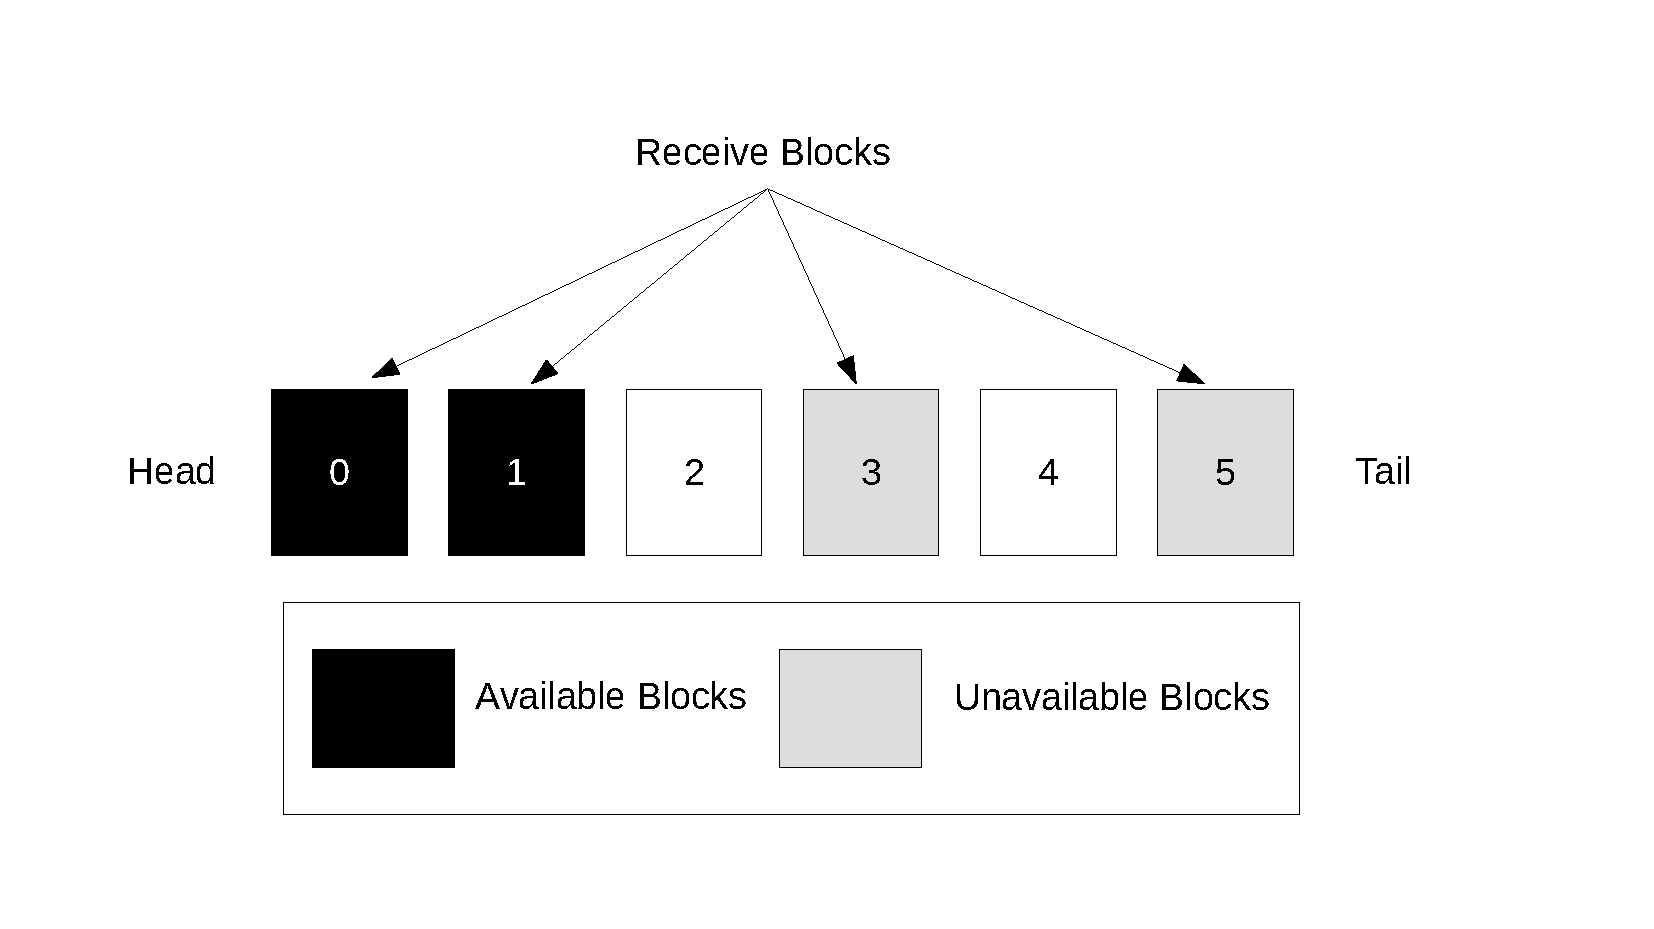
\includegraphics[width=18cm]{block.pdf}
\caption{ブロックの有効性}
\label{block}
\end{figure}

 %%%%%%%%%%%%%
 \section{重複再要求}
 \label{juhuku}
 \ref{hukusu}節で述べた性能差のある複数のTCP接続を用いたプログレッシブダウンロードにおいて起こりうる問題点を,アプリケーション層での制御で解消するために提案されている方式として,重複再要求[]がある.この方式では未取得ブロックより後に合計N個以上(有効・非有効は問わない)のブロックがあれば,未取得ブロックをその未取得ブロックを要求したTCP接続とは別のTCP接続へ再要求を行う.図\ref{blockdup}にその模式図を示す.図\ref{blockdup}の例では重複再要求を行い,ブロック2を取得することで少なくともでもブロック3が非有効ブロックである状態を解消することができる.この操作を受信イベントが発生するたびに繰り返すことで,バッファ上の非有効ブロックの個数の増加を抑制することができ,応答性の向上が見込まれる.
 
 \begin{figure}[h]
     \centering
     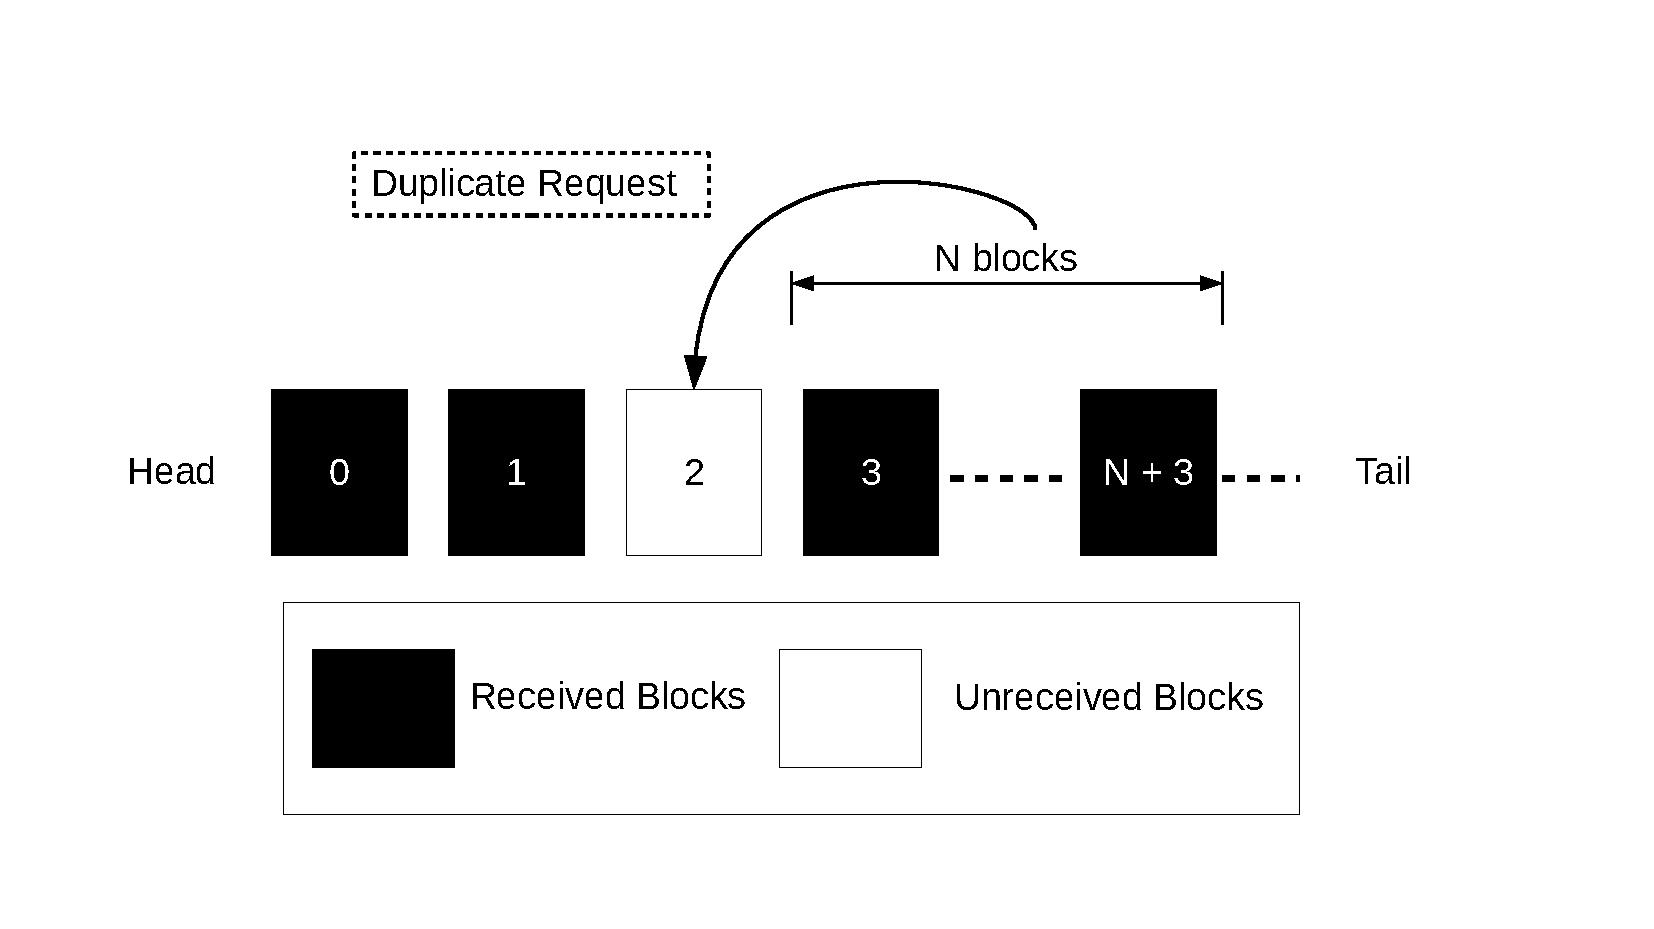
\includegraphics[width=18cm]{block_dup.pdf}
     \caption{重複再要求の模式図}
     \label{blockdup}
 \end{figure}

\newpage
 
 
 \section{タイマ駆動を用いた要求方式}
 \ref{hukusu}節で述べた複数のTCP接続を用いたプログレッシブダウンロードにおいて起こりうる問題点を解消するために提案されている方式として,タイマ駆動型要求方式[]がある.\ref{juhuku}節で述べた重複再要求方式は,ブロックの遅延に対して後から対処するという方針であるが,本節で述べるタイマ駆動を用いた要求方式は,TCP接続の性能差を予め考慮することで,到着順序逆転の発生そのものを抑制しようという方針である.
 タイマ駆動
 
\chapter{提案方式}\label{sec:sec3}
本章では性能差のある複数のTCP接続を並列的に利用する際に生じうるいくつかの問題点を解消するためのアルゴリズムを実装した提案方式について述べる.\\
また,実際に複数のTCP接続を用いた動画のプログレッシブダウンロードをプログラムに実装する際に考慮すべき点がいくつかある.プログレッシブダウンロードの実装は大きく分けて動画ファイルのダウンロードとバイナリファイルをデコードして再生という2つのセクションに分かれている.既存のウェブブラウザやVLC[]等のネットワークメディア再生機能付きの動画プレイヤーソフトのではこの2つのセクションは1つのプログラムから高度に同期をとりながら同時並列的に制御されている.しかし,本研究では実装の難易度と主としてダウンロードセクションについて論じるためにこれら2つのセクションは分離している.

\section{遅延要求方式}
\label{chienyokyuhoshiki}
\ref{chienyokyu}節では遅延要求の概要について述べる.
\ref{kotei}節では各接続の帯域が既知であるいう仮定に基づいて,TCP接続の性能差を入力し,ブロックの要求位置を変化させることで到着順序逆転の抑制する方式について提案する.
\ref{diff}節では未知のネットワーク状況に対応するためにTCP接続の使用回数の差分に注目しブロックの遅延度を推測する方式について提案する.

\subsection{遅延要求について}
\label{chienyokyu}
この章で定義する遅延要求についての概要を述べる.まず,確立したTCP接続群の中で性能の最も高いTCP接続には,最も若番のブロックを要求する.
続いて,比較性能の低いあるTCP接続に関して,ブロック要求の送信からブロックの到着までの間隔を算出し,
その算出値に基づいてその時点での最も若番のブロックではない後ろのブロックを要求する.
図\ref{delay}にその模式図を示す.この例では,接続Aは接続Bの2倍の性能を持つと仮定する.
この条件より接続Bがブロックを1個取得する間に接続Aはブロックを2個取得取得することが予想できる.
よって時刻t=0に接続Aにはブロック0を要求し,接続Bにはブロック2を要求する.
t=1には接続Aにブロック番号0が到着し,続いて接続Aがにブロック1を要求する.
時刻t=2において接続Aには2より若い番号のブロックが到着済みであり,接続Bはブロック2の取得が完了する.
よってブロックの到着順序逆転を抑制することができる.
\ref{kotei}節ではあらかじめ各接続間の性能差が既知であるとして,その値にしたがって遅延要求を行う方式について述べる.
\ref{diff}節では各接続ごとにブロック到着間隔を逐次測定することで性能差を算出し,その値にしたがって遅延要求を行う方式について述べる.

 \begin{figure}[h]
    \centering
    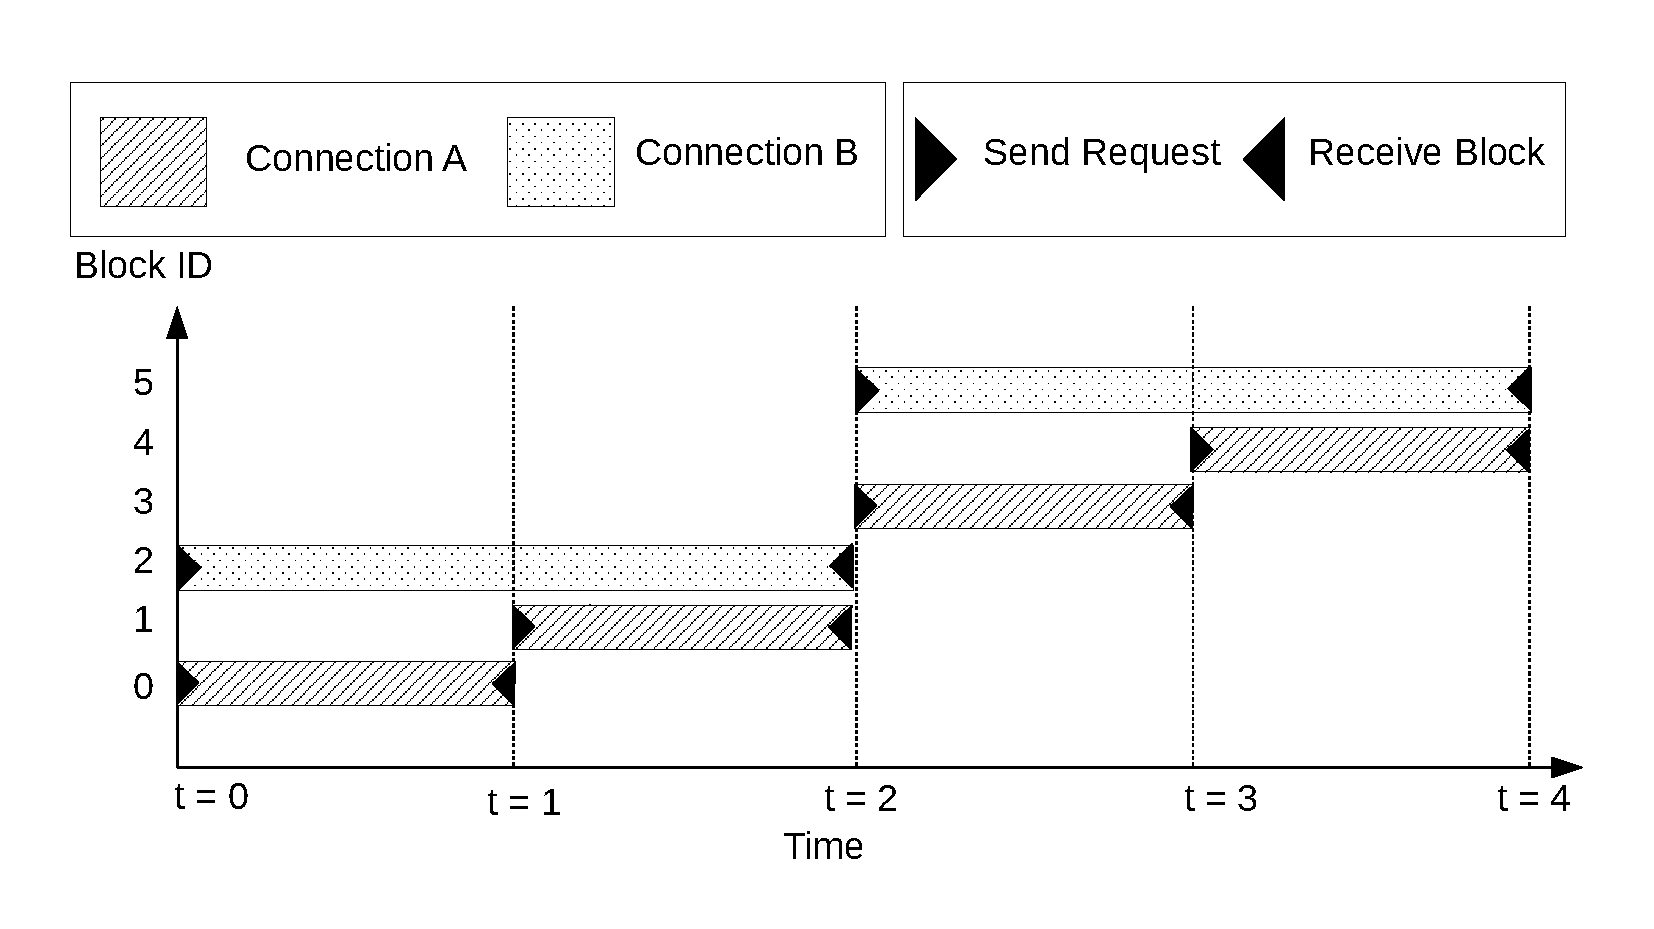
\includegraphics[width=16.25cm]{delay.pdf}
    \caption{遅延要求の模式図}
    \label{delay}
\end{figure}

\subsection{固定遅延要求方式}
\label{kotei}
固定遅延方式は,予めTCP接続間の性能差をシステムに入力して遅延要求を行うことで到着順序逆転の抑制を試みる方式である.しかし,実ネットワークでは予めTCP接続間の性能差が既知であることは稀であるので実環境への応用は限定的であると言わざるを得ない.よって本研究では本方式は主として,他の方式がどれだけTCP接続間の性能差を正確に把握できているかどうかを比較し確認するために用いる.

\subsection{差分計測を用いた遅延予測方式}
\label{diff}
当方式はあるTCP接続に対して何ブロック後ろのブロックを要求するかを算出するために,そのTCP接続の直前のブロック取得間隔を計測し用いる方式である.以下に疑似コードを示す.最も性能の高いTCP接続には0を割り当てる.

\begin{algorithm}
	\caption{Compute Diff}
	\begin{algorithmic}[1]
		\State {$T \gets Total\ Receive\ Count$}
		\State {$P \gets Previous\ Receive\ Counts $}
		\State {$N \gets Number\ Of\ Connections$}
		\If{Is it the highest performance} 
		\State {$D \leftarrow 0$}
		\Else 
		\State {$D \leftarrow T - P - N $}
		\EndIf
	\end{algorithmic}
	
\end{algorithm}

\section{初期遅延予測}
\label{shoki}
\ref{diff}節の遅延要求方式は実装上の都合,最初のリクエスト送信の際にはTCP接続間の性能差が不明であるため,遅延要求を行うことができない.しかし実際にエンドユーザーが動画再生を行うことを想定すると,初期バッファリング時間の長さは視聴体験に大きく影響を及ぼすことが予想される.本節ではこの問題の解決案として初期値を予測し初期バッファリング時間の短縮を目指す方式を提案する.

\subsection{概要}
\label{shokigaiyo}
\ref{chienyokyuhoshiki}節の遅延要求方式ではファイル情報を取得するために,事前にHTTPのHEADリクエストを相手サーバーに送信している.このHEADリクエストの応答時間を計測することで,各TCP接続間の性能差も推測できる.ただし,後続のGETリクエストの応答メッセージサイズはHEAD レスポンスのそれよりも大きく,実際には一つのHTTPレスポンスに対して複数のTCPセグメントがやり取りされるので,厳密な意味での応答時間ではなく単一のHEAD レスポンスの応答時間であることに注意が必要である.

\subsection{予測方法}
\label{yosokuhouhou}
本節では具体的な予測アルゴリズムについて述べる.初期遅延度は各TCP接続において計測したHEAD リクエストの応答時間と,すべてのTCP接続の応答時間の最小値との比を用いて算出する.以下に疑似コードを示す.

\begin{algorithm}
	\caption{Compute Initial Delays}
	\begin{algorithmic}[1]
		\State {$R \gets Raw\ Delays $}
		\State {$M \gets MIN(R)$}
		\State {$D \gets Delays $}A
		\State {$C \gets Coefficient$}
		\ForAll {r in R}
		\State {$d \leftarrow r \ / \  M \ * \ C$}
		\State {$Add\ d\ to\ D$}
		\EndFor
	\end{algorithmic}
	
\end{algorithm}


\chapter{実装評価}\label{sec:sec4}

本章では提案方式を実装し,評価する.

\section{重複再要求方式}
本評価では重複再要求方式として\ref{juhuku}を改良し非有効ブロックの受信回数を閾値として用いる.これは実装上の都合であり,関連研究のアルゴリズムとは若干異なるが本研究では重複再要求のアルゴリズムを比較することは目的としていない.

\section{評価項目}
\label{hyoukakoumoku}
本章で評価する評価値について整理する.
\begin{table}[htb]
	\begin{center}
		\caption{評価項目}
		\begin{tabular}{|c|c|} \hline
			評価項目 & 概要 \\ \hline \hline
			平均遅延時間 & ブロックの理想的な到達時刻からどれだけ遅れているか\\ \hline
			初期バッファリング時間 & 初期バッファリングに必要な時間 \\ \hline
			平均非有効ブロック数 & バッファ内の非有効ブロックの数 \\ \hline
			
		\end{tabular}
	\end{center}
\end{table}

\newpage

\section{テストベッドでの評価}
\label{testbed}
\ref{networkmodel}にネットワークモデルを示す.TCP接続A-TCP接続B間の性能差は3倍,TCP接続A-TCP接続C間の性能差は10倍である.
\begin{figure}[h]
	\label{networkmodel}
	\begin{center}
		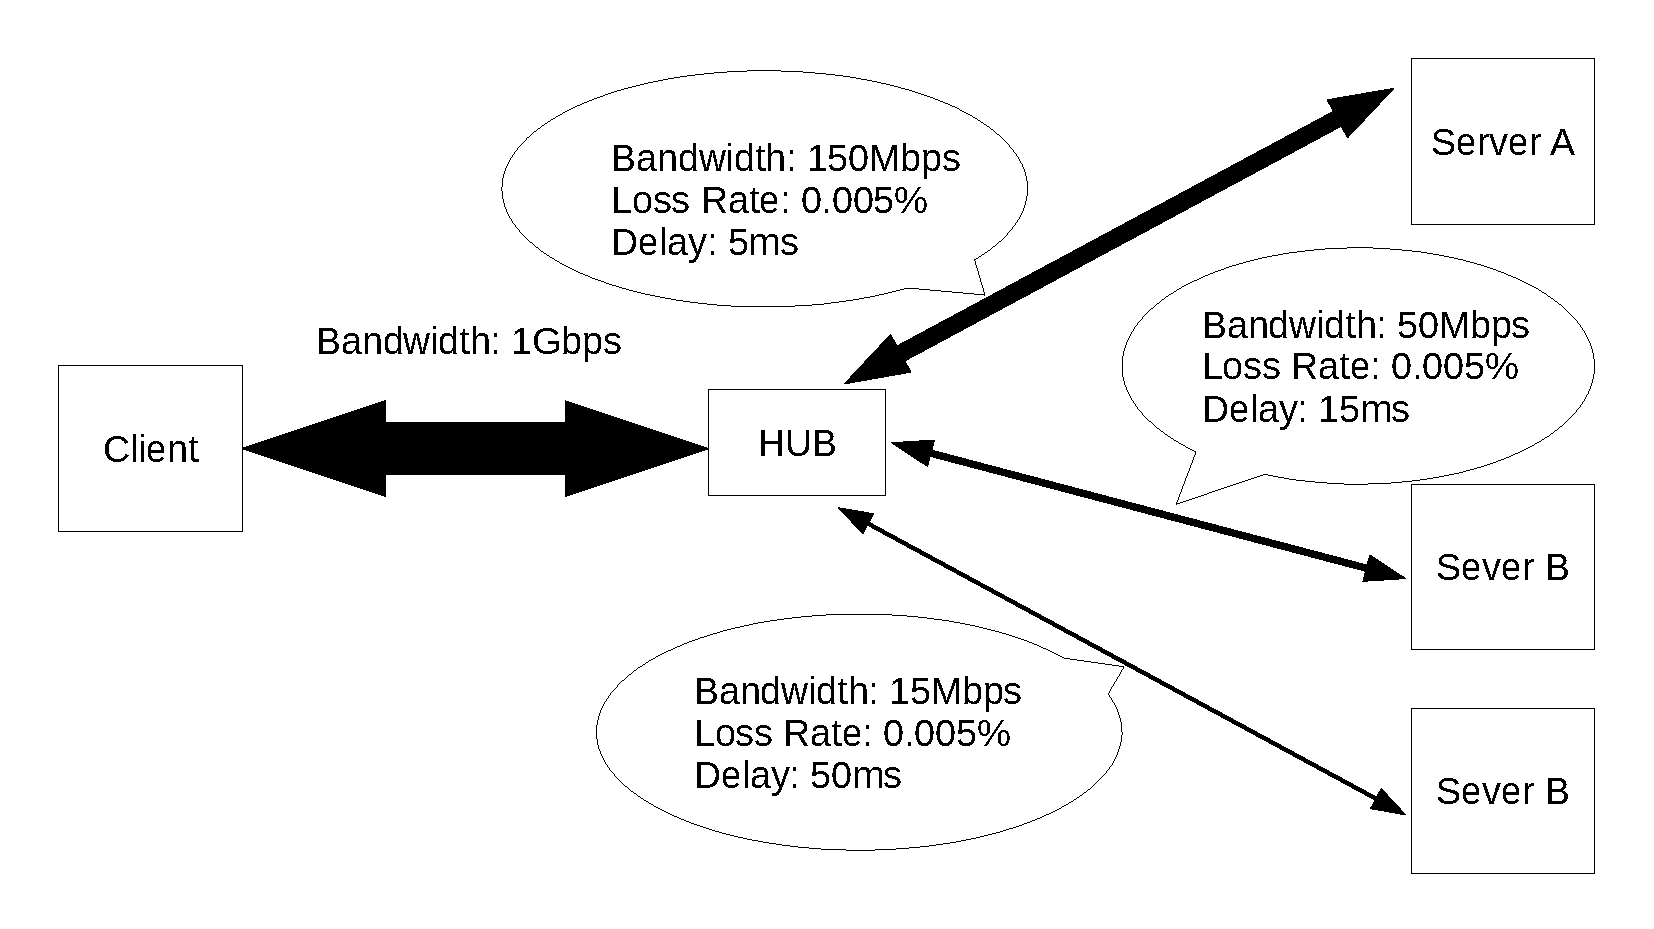
\includegraphics[width=16cm]{test_network.pdf}
		\caption{ネットワークモデル}
	\end{center}
\end{figure}

\begin{table}[htb]
	\begin{center}
		\caption{実験環境}
		\begin{tabular}{|c|c|} \hline
			ファイルサイズ & 754MB\\ \hline
			ファイル &  ubuntu-17.10.1-server-amd64.iso\\ \hline
			OS(Server and Client) & ubuntu 17.10 (Kernel 4.13)\\ \hline
			TCP & CUBIC \\ \hline
			HTTP Server & h2o v2.2.4 \\ \hline
		\end{tabular}
	\end{center}
\end{table}

\newpage

\begin{figure}[h]
	\begin{center}
		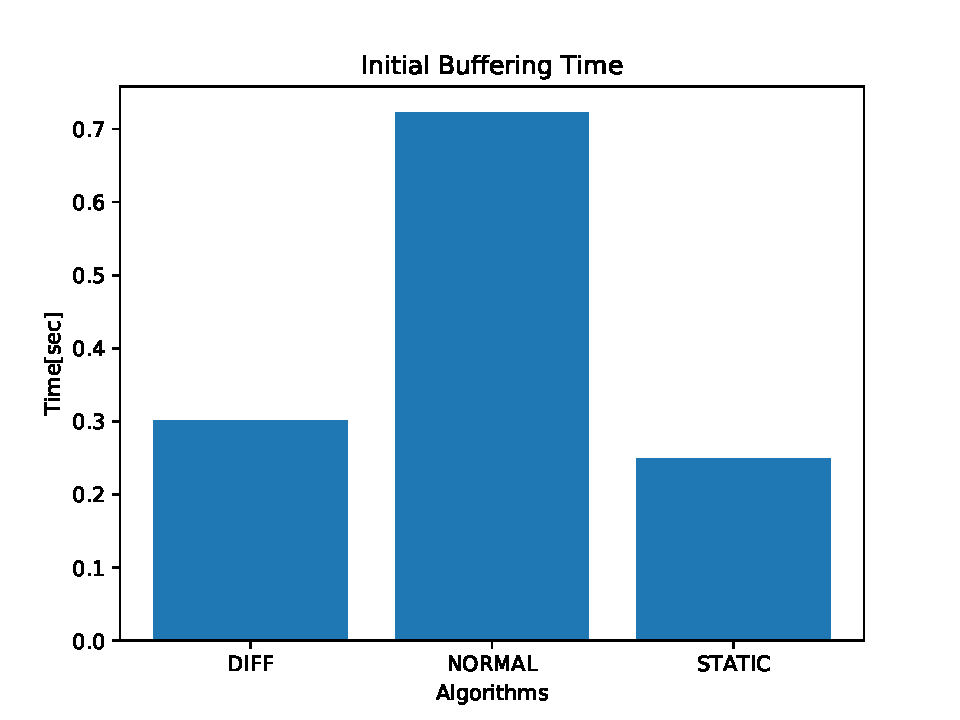
\includegraphics[width=15cm]{InitialBufferingTime.pdf}
		\caption{初期バッファリング時間}
		\label{ibt}
	\end{center}
\end{figure}
図\ref{ibt}は遅延要求のアルゴリズムごとの初期バッファリング時間である.DIFFは差分計測を用いた遅延要求方式,NORMALは常時最若番を要求する方式(制御を何も行わない),STATICはTCP接続間の性能差を入力する固定遅延要求方式である.図\ref{ibt}より差分計測を用いた遅延要求方式はTCP接続間の性能差を入力することなく固定遅延要求方式に近い性能を獲得できていると言える.

\newpage

\begin{figure}[h]
	\begin{center}
		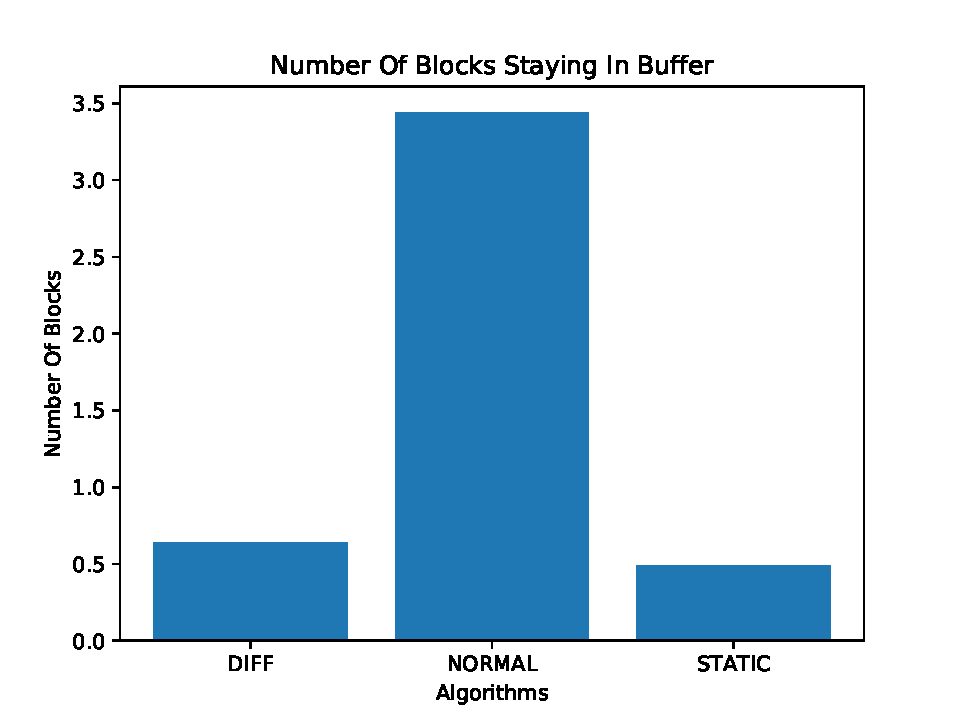
\includegraphics[width=15cm]{NumberOfBlocksStayingInBuffer.pdf}
		\caption{非有効ブロック数}
		\label{nsb}
	\end{center}
\end{figure}

図\ref{nsb}は遅延要求のアルゴリズムごとの初期バッファリング時間である.DIFFは差分計測を用いた遅延要求方式,NORMALは常時最若番を要求する方式(制御を何も行わない),STATICはTCP接続間の性能差を入力する固定遅延要求方式である.図\ref{ibt}より差分計測を用いた遅延要求方式はTCP接続間の性能差を入力することなく固定遅延要求方式に近い性能を獲得できていると言える.

\newpage

\section{公開ネットワークでの評価}
\label{pub}
公開ネットワークでの評価にあたりUbuntuのパブリックミラーを利用した.\ref{tablemirror}に使用したパブリックミラーを示す.また,参考として各パブリックミラーの24時間の性能変化について図\ref{24h}に示す
\begin{table}[htb]
	\begin{center}
		\caption{使用したパブリックミラー}
		\label{tablemirror}
		\begin{tabular}{|l|l|l|} \hline
			ホスト & 組織 & 国\\ \hline \hline
			ftp.jaist.ac.jp & JAIST & JP \\
			ubuntutym2.u-toyama.ac.jp & Univercity of Toyama & JP \\
			releases.ubuntu.com & Canonical & GB \\
			mirrorservice.org & University of Kent & GB \\
			ubuntu.ipacct.com & IPACCT & BG \\
			mirror.enzu.com & Enzu Inc. & US \\
			mirror.pop-sc.rnp.br & PoP-SC & BR \\
			ftp.belnet.be & Belnet & BE \\
			mirrors.mit.edu & MIT & US \\
			mirror.yandex.ru & Yandex & RU \\ \hline
		\end{tabular}
	\end{center}
\end{table}

\begin{figure}[h]
    \begin{center}
        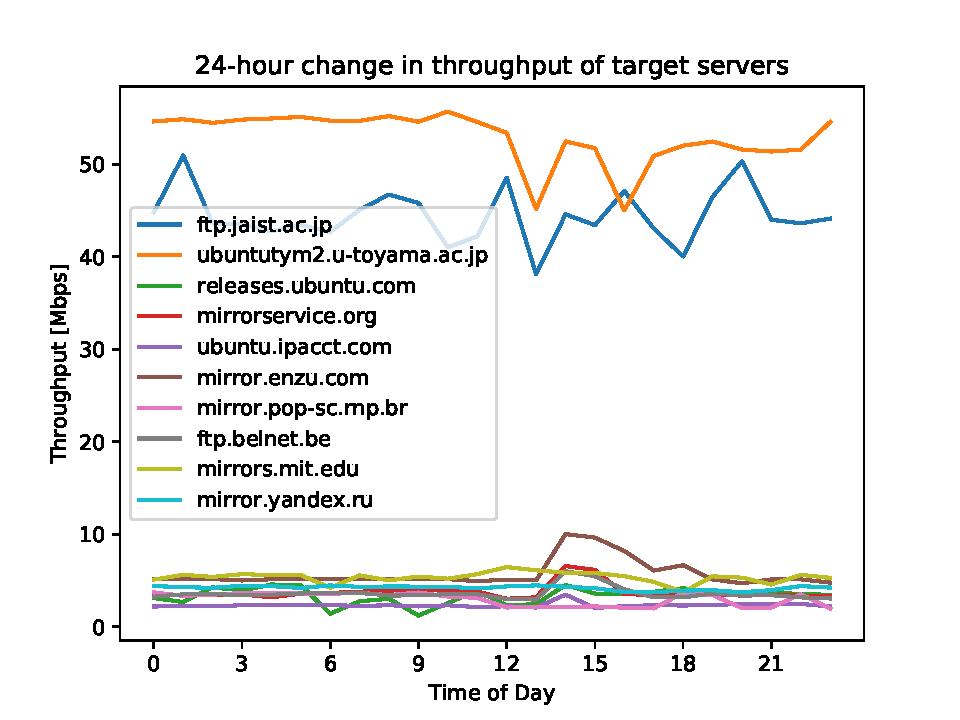
\includegraphics[width=12cm]{thp24h.pdf}
        \caption{各パブリックミラーの24時間の性能の変化}
        \label{24h}
    \end{center}
\end{figure}

\newpage
 
%%%%%%%%%%%%%%%%%%%%%%%%%%%%%%%%%%%%%%%%%%%%%%%%%%%%%%%%%%%%%%%%%%%%%%%%%%%%
% 第X章
%%%%%%%%%%%%%%%%%%%%%%%%%%%%%%%%%%%%%%%%%%%%%%%%%%%%%%%%%%%%%%%%%%%%%%%%%%%%%
\chapter{今後の課題}\label{sec:sec7}
\hspace*{0.5em}今後の課題として, 以下が挙げられる.
\begin{itemize}
    \item 実際のユーザー体験を考慮した評価
    \item タイマ駆動要求方式の実装との比較
\end{itemize}

\chapter{付録}
\section{ソースコード}
本研究で実装したソースコードはすべてGitHubにて公開している.\\
\url{https://github.com/johejo/sphttp}
\section{プロキシのプロトタイプを用いた実装}

\clearpage
%
%%%%%%%%%%%%%%%%%%%%%%%%%%%%%%%%%%%%%%%%%%%%%%%%%%%%%%%%%%%%%%%%%%%%%%%%%%%%%
% 謝辞
%%%%%%%%%%%%%%%%%%%%%%%%%%%%%%%%%%%%%%%%%%%%%%%%%%%%%%%%%%%%%%%%%%%%%%%%%%%%%
\begin{acknowledgment}
 本研究の機会を与えて頂き,多くの御指導,および御助言を賜わりました
舟阪 淳一 准教授に深甚なる謝意を表します.また,その他多くの御助言を頂きま
した諸氏に心より感謝致します.
\end{acknowledgment}
%%%%%%%%%%%%%%%%%%%%%%%%%%%%%%%%%%%%%%%%%%%%%%%%%%%%%%%%%%%%%%%%%%%%%%%%%%%%%
% 参考文献
%%%%%%%%%%%%%%%%%%%%%%%%%%%%%%%%%%%%%%%%%%%%%%%%%%%%%%%%%%%%%%%%%%%%%%%%%%%%%
\begin {thebibliography}{20} 
\bibitem{test} test

\end {thebibliography}

\end{document}
